\documentclass[11pt,a4paper]{article}
\usepackage[margin=2.2cm]{geometry}
\usepackage{amsmath,amssymb,booktabs,array,graphicx,float,microtype}
\usepackage[dvipsnames]{xcolor}
\usepackage[hidelinks]{hyperref}
\usepackage{fancyhdr}
\usepackage{enumitem}
\usepackage{caption}
\usepackage{longtable}

\definecolor{navy}{HTML}{16324F}
\definecolor{teal}{HTML}{2A9D8F}
\definecolor{orange}{HTML}{E76F51}
\definecolor{light}{HTML}{F3F6F8}
\hypersetup{colorlinks=true,linkcolor=navy,urlcolor=teal,citecolor=navy}
\graphicspath{{figures/stability_topology/}}
\pagestyle{fancy}
\fancyhf{}
\lhead{Adaptive Governance Stability Study}
\rhead{Independent Computational Report}
\cfoot{\thepage}
\setlength{\headheight}{14pt}
\setlist[itemize]{leftmargin=1.4em,itemsep=0.3em}
\captionsetup{font=small,labelfont=bf}

\newcommand{\code}[1]{\texttt{#1}}
\newcommand{\good}[1]{\textcolor{teal}{\textbf{#1}}}
\newcommand{\warn}[1]{\textcolor{orange}{\textbf{#1}}}

\begin{document}

\begin{titlepage}
\centering
\vspace*{1.2cm}
{\color{navy}\rule{\textwidth}{1.3pt}}\\[1.1cm]
{\Huge\bfseries Local Stability and Topological Structure\\[0.3cm]
of an Adaptive DeFi Risk Controller\par}
\vspace{0.6cm}
{\Large A 360-point parameter-neighbourhood experiment\par}
\vspace{1.0cm}
{\large Niko Rokni Lamouki \quad and \quad Salma Soofiyan\par}
\vfill
\begin{minipage}{0.84\textwidth}
\colorbox{light}{\parbox{0.94\textwidth}{
\textbf{Scope.} This report tests whether convergent controller coefficients
form a robust local neighbourhood and whether the sampled stable set has a
detectable topological structure. It combines a reduced-order closed-loop
stability probe, 138,240 four-month economic paths, and persistent homology with
a matched random-cloud null test. It is computational evidence, not a formal
Lyapunov proof or a production deployment claim.
}}
\end{minipage}
\vfill
{\large Experiment seed: \code{20261105}\\[0.2cm]
Repository: \url{https://github.com/nikorokni/local-currency-defi-adaptive-governance}}
\vspace{0.7cm}
{\color{navy}\rule{\textwidth}{1.3pt}}
\end{titlepage}

\pagenumbering{roman}
\tableofcontents
\clearpage
\pagenumbering{arabic}

\section{Executive summary}

The published controller uses fixed coefficients in a bounded, rate-limited
map from observed volatility, DEX basis, oracle disagreement, and utilisation
to the borrowing rate, debt ceiling, liquidation ratio, and circuit-breaker
state. The original simulations establish economic performance under common
shocks, but they do not show whether one successful coefficient vector is
surrounded by other convergent vectors.

This report provides that missing computational experiment. A 96-point broad
Latin-hypercube pilot located a stable centre. Exactly 360 stratified random
points were then sampled around that centre. Each point was tested from nine
perturbed initial states in six stability cases (three stress regimes, each at
zero and 48-hour delay), and was separately run on 192 common ARS paths and 192
common TRY paths.

\begin{center}
\begin{tabular}{>{\raggedright\arraybackslash}p{0.48\textwidth}r}
\toprule
Headline result & Value\\
\midrule
Broad pilot points robustly convergent & 11 / 96\\
Local points robustly convergent & \good{360 / 360}\\
Local points converging in all six cases & 261 / 360\\
Four-month economic paths in local stage & 138,240\\
Median pooled bad-debt-event probability & 0.2604\%\\
Local stable-set components at connection scale & 1\\
Observed maximum $H_1$ persistence & 0.1844\\
Matched-null $p$-value for maximum $H_1$ persistence & 0.9355\\
Evidence of non-trivial one-dimensional hole & \warn{No}\\
\bottomrule
\end{tabular}
\end{center}

The evidence supports a connected local stability basin. It does not support a
robust ring or hole after comparison with uniform eight-dimensional
Latin-hypercube clouds. Stability is not identical to economic safety: TRY
severe depegs remain in the common-path experiment even when controller states
converge.

\section{Controller and parameter space}

\subsection{Parameterised equations}

The experiment preserves the published baseline by exposing eight coefficients
that had previously appeared as literals. The EWMA variance is
\begin{equation}
v_{t+1}=\beta v_t+(1-\beta)q_t^2,
\end{equation}
and the composite risk score is
\begin{equation}
R_t=\operatorname{clip}_{[0,1]}\left(
w_\sigma\sqrt{v_{t+1}}+w_b b_t+w_\delta\delta_t+
w_u(u_t-0.72)_+\right).
\end{equation}
The three parameter targets are
\begin{align}
r_t^*&=\operatorname{clip}_{[0.04,1.50]}
\left(0.08+g_rR_t+0.35(u_t-0.75)_+\right),\\
C_t^*&=\operatorname{clip}_{[0.20,1.00]}\left(e^{-g_CR_t}\right),\\
\lambda_t^*&=\operatorname{clip}_{[1.50,2.20]}
\left(1.50+g_\lambda R_t\right).
\end{align}
The published per-step movement bounds remain unchanged. Therefore setting
\(\theta\) to the baseline row in Table~\ref{tab:parameters} reproduces the
original equations exactly.

\subsection{Parameter collection}

\begin{table}[H]
\centering
\caption{Influential controller coefficients and broad search intervals.}
\label{tab:parameters}
\begin{tabular}{llll}
\toprule
Coefficient & Symbol & Baseline & Broad interval\\
\midrule
EWMA memory & $\beta$ & 0.92 & $[0.80,0.98]$\\
Volatility weight & $w_\sigma$ & 4.00 & $[2.50,5.50]$\\
DEX-basis weight & $w_b$ & 3.20 & $[2.00,4.50]$\\
Disagreement weight & $w_\delta$ & 1.80 & $[1.00,2.80]$\\
Utilisation weight & $w_u$ & 0.90 & $[0.40,1.40]$\\
Rate response gain & $g_r$ & 0.90 & $[0.50,1.30]$\\
Ceiling response gain & $g_C$ & 1.75 & $[0.80,2.80]$\\
Liquidation response gain & $g_\lambda$ & 0.70 & $[0.35,1.10]$\\
\bottomrule
\end{tabular}
\end{table}

The selected pilot centre was
\begin{equation}
\hat\theta=(0.94569,3.17732,2.31667,1.48870,
0.70887,0.52487,0.81518,0.57902).
\end{equation}
It is a centre for local robustness sampling, not a claimed economic optimum.

\section{Experimental design}

\begin{figure}[H]
\centering
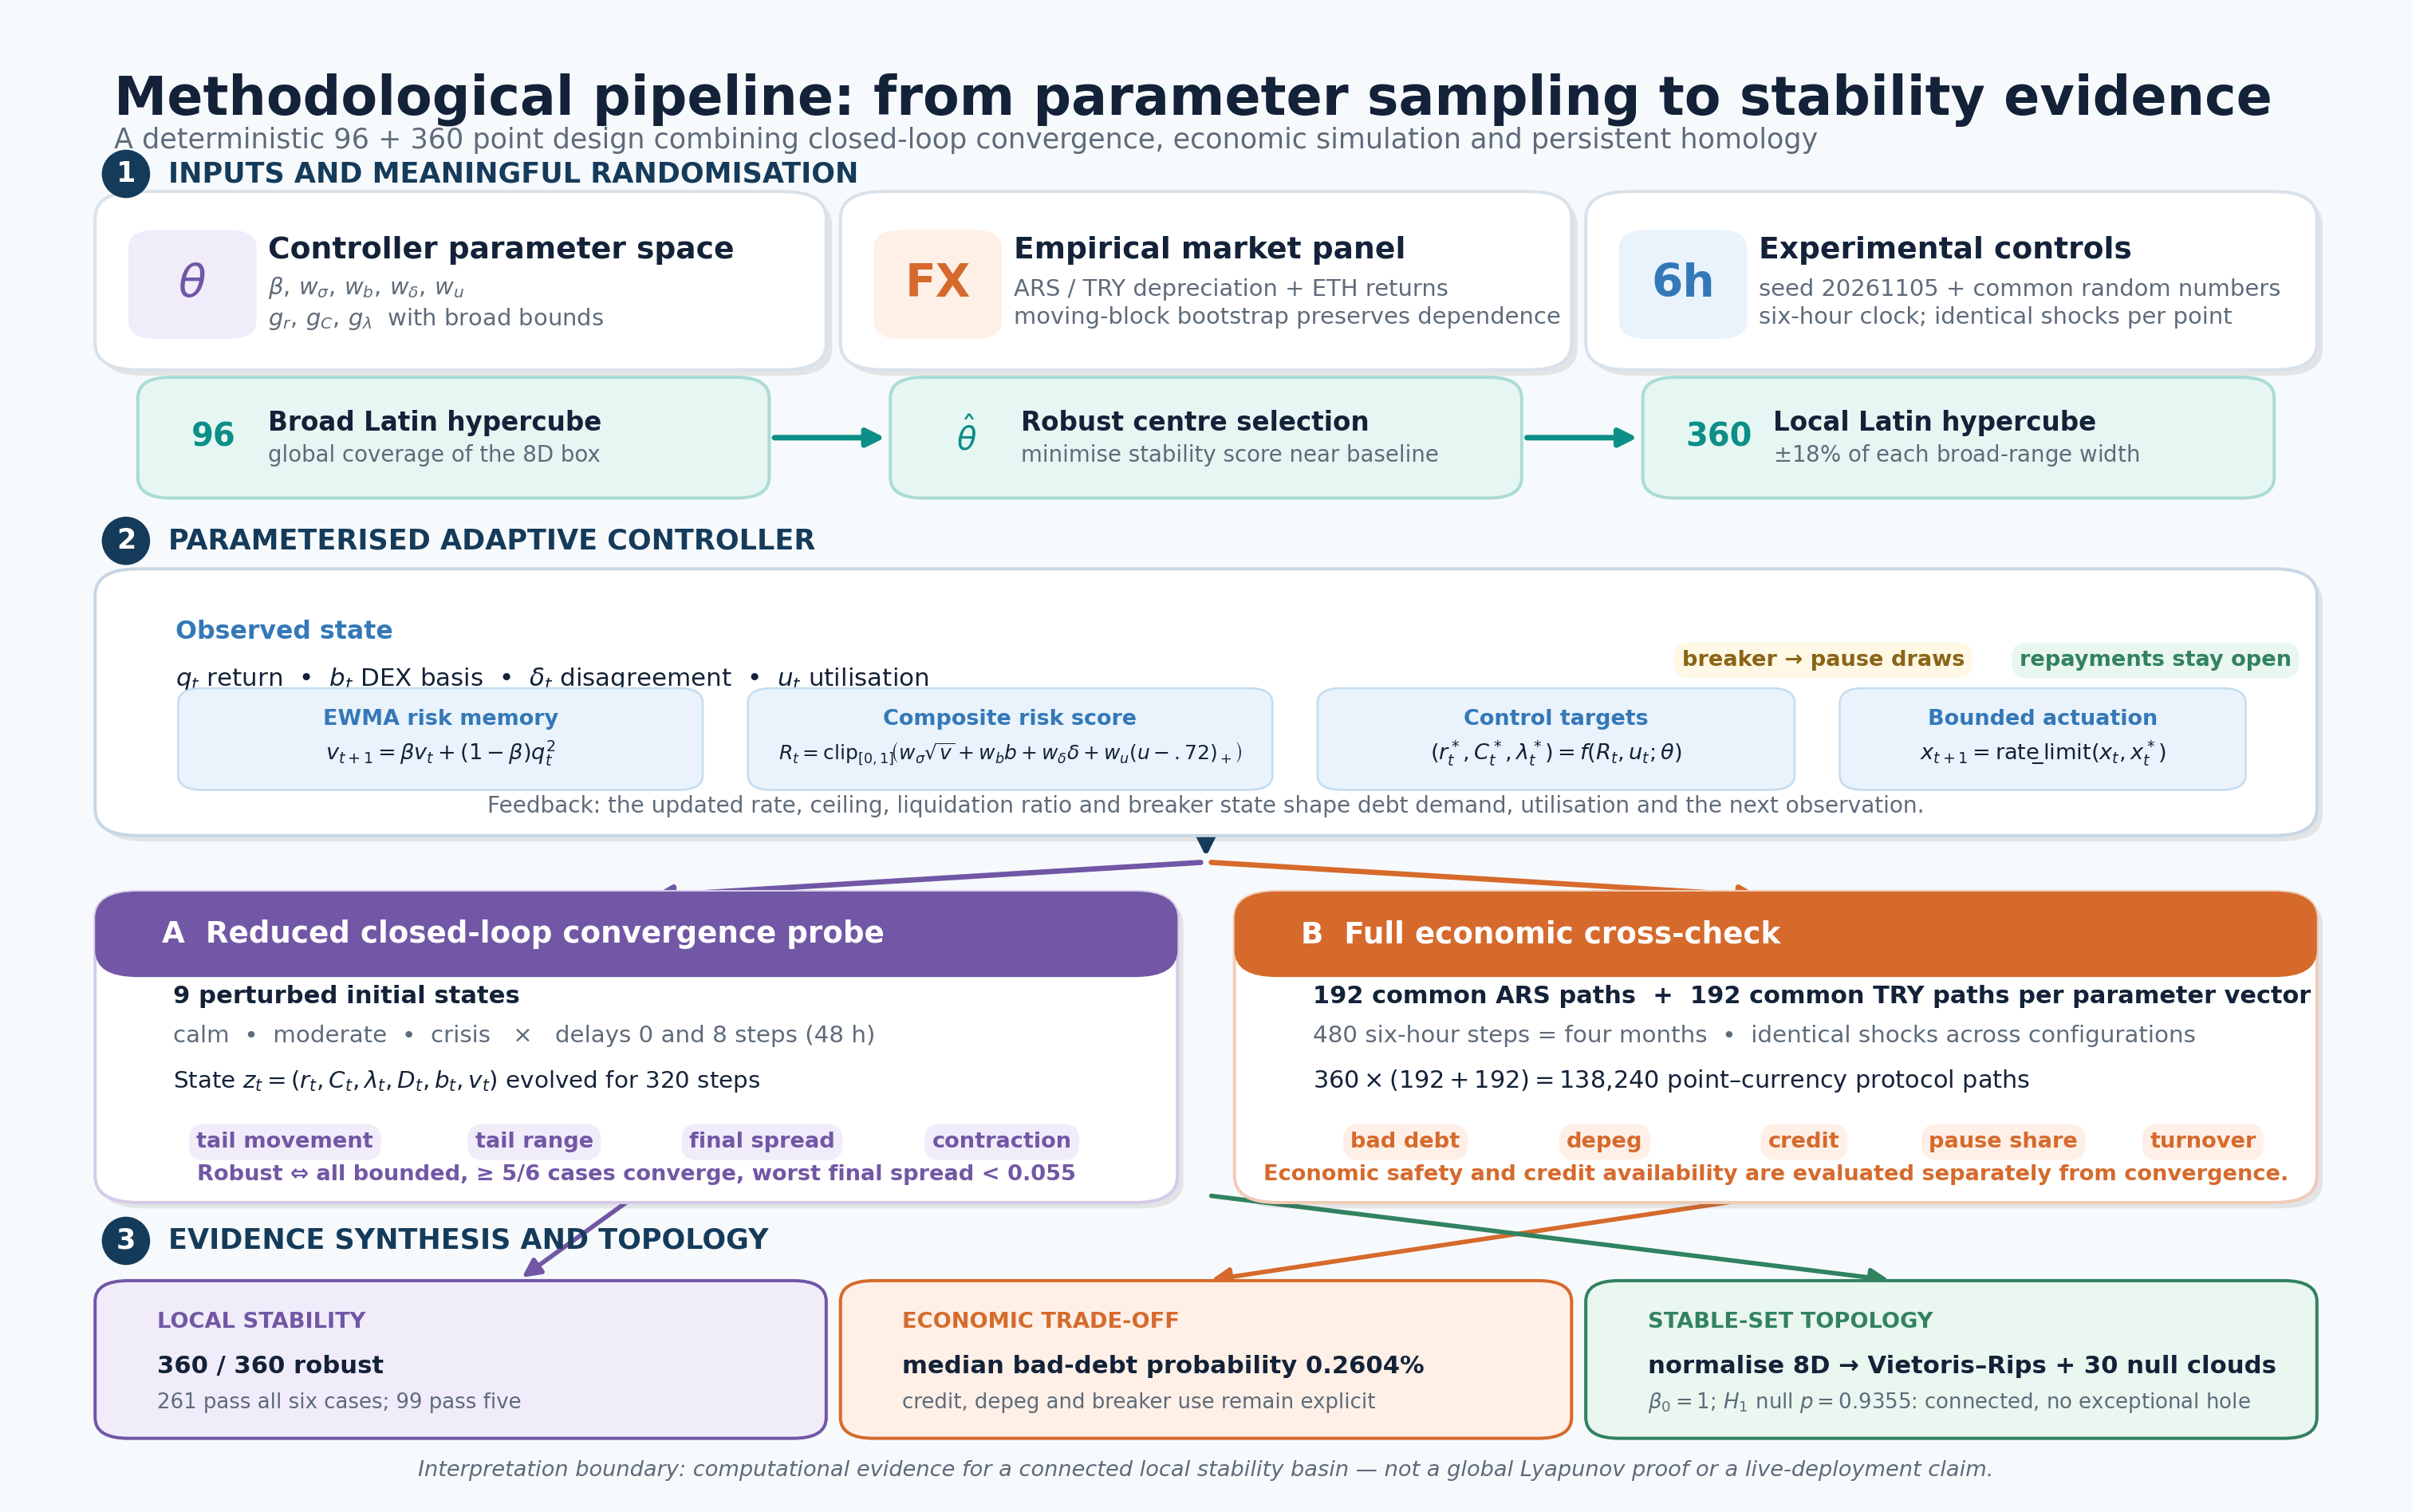
\includegraphics[width=\textwidth]{figure6_methodology_pipeline.png}
\caption{End-to-end methodology. Broad parameter sampling and common market
inputs feed the parameterised controller. Every local vector is then evaluated
through a reduced closed-loop convergence probe and a full economic simulation
before stability, economic, and topological evidence are synthesised.}
\label{fig:methodology-pipeline}
\end{figure}

\subsection{Meaningful random sampling}

Independent uniform draws can cluster and leave large gaps. We instead use a
deterministic Latin-hypercube design: every parameter marginal is divided into
equal-probability strata and each stratum is visited once. A 96-point pilot
covers the broad box. A second 360-point design covers a neighbourhood equal to
18\% of each broad-range width on either side of the stable centre, clipped to
the broad bounds. All randomisation is controlled by seed \code{20261105}.

\subsection{Reduced closed-loop stability probe}

The stability state is
\begin{equation}
z_t=(r_t,C_t,\lambda_t,D_t,b_t,v_t),
\end{equation}
where demand responds negatively to the rate and available ceiling, debt
accrues interest and is repaid, DEX basis responds to accepted draws and
arbitrage capacity, and the breaker can pause new draws. This reduced model
preserves the feedback signs, hard domains, step bounds, and breaker asymmetry of
the full simulator.

Nine perturbed initial states are evaluated in calm, moderate, and crisis
regimes. Each regime is run both without delay and with an eight-step (48-hour)
delay. A case passes only if all state variables remain finite and in-domain and
if
\begin{align}
\overline{\lVert z_t-z_{t-1}\rVert}_{\mathrm{tail}}&<0.002,\\
\operatorname{range}_{\mathrm{tail}}(z)&<0.030,\\
\operatorname{spread}(z_T)&<0.040,\\
\operatorname{spread}(z_T)/\operatorname{spread}(z_0)&<0.50.
\end{align}
A vector is robustly convergent when all six cases remain bounded, at least five
cases pass, and the worst terminal spread is below 0.055.

\subsection{Full economic cross-check}

Every local point is evaluated with the full lending-book simulator on 192 ARS
and 192 TRY four-month paths, each containing 480 six-hour steps. The same
market paths are reused for every point. This common-random-number design removes
shock-sampling variation from comparisons between parameter vectors.

\section{Stability results}

Only 11 of the 96 broad pilot points passed the robust criterion. The published
baseline remained bounded but converged in four of six reduced cases; it failed
the stricter cross-perturbation contraction requirement. This should not be read
as proof that the published finite-horizon economic simulation is unstable.
Rather, it identifies a gap between finite-path performance and local-attractor
evidence under the additional frozen-regime tests.

All 360 local points passed the robust criterion. Of these, 261 passed all six
cases and 99 passed five. The local cloud therefore supplies evidence that the
selected convergent values are not isolated.

\begin{figure}[H]
\centering
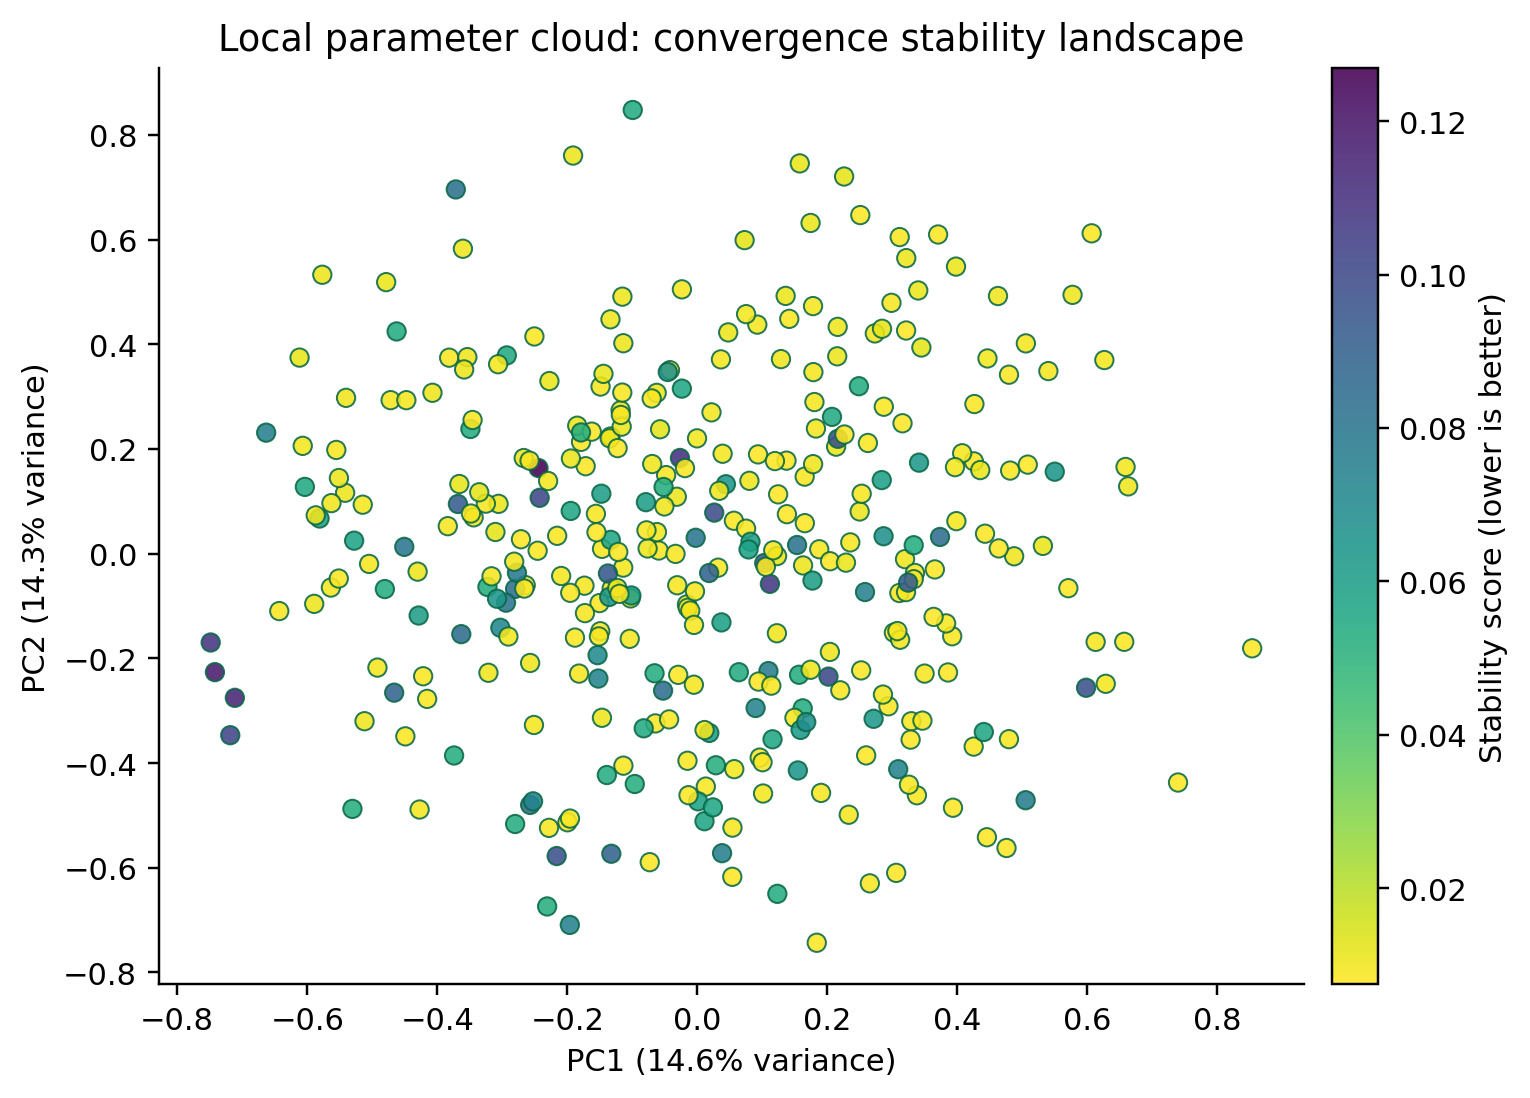
\includegraphics[width=0.88\textwidth]{figure1_parameter_cloud_pca.png}
\caption{PCA view of the eight-dimensional local cloud. Edge colour denotes the
robust label; fill colour is the continuous stability score. The first two PCs
explain only 28.9\% of parameter variance, so this plot is illustrative rather
than a complete representation of geometry.}
\end{figure}

\begin{figure}[H]
\centering
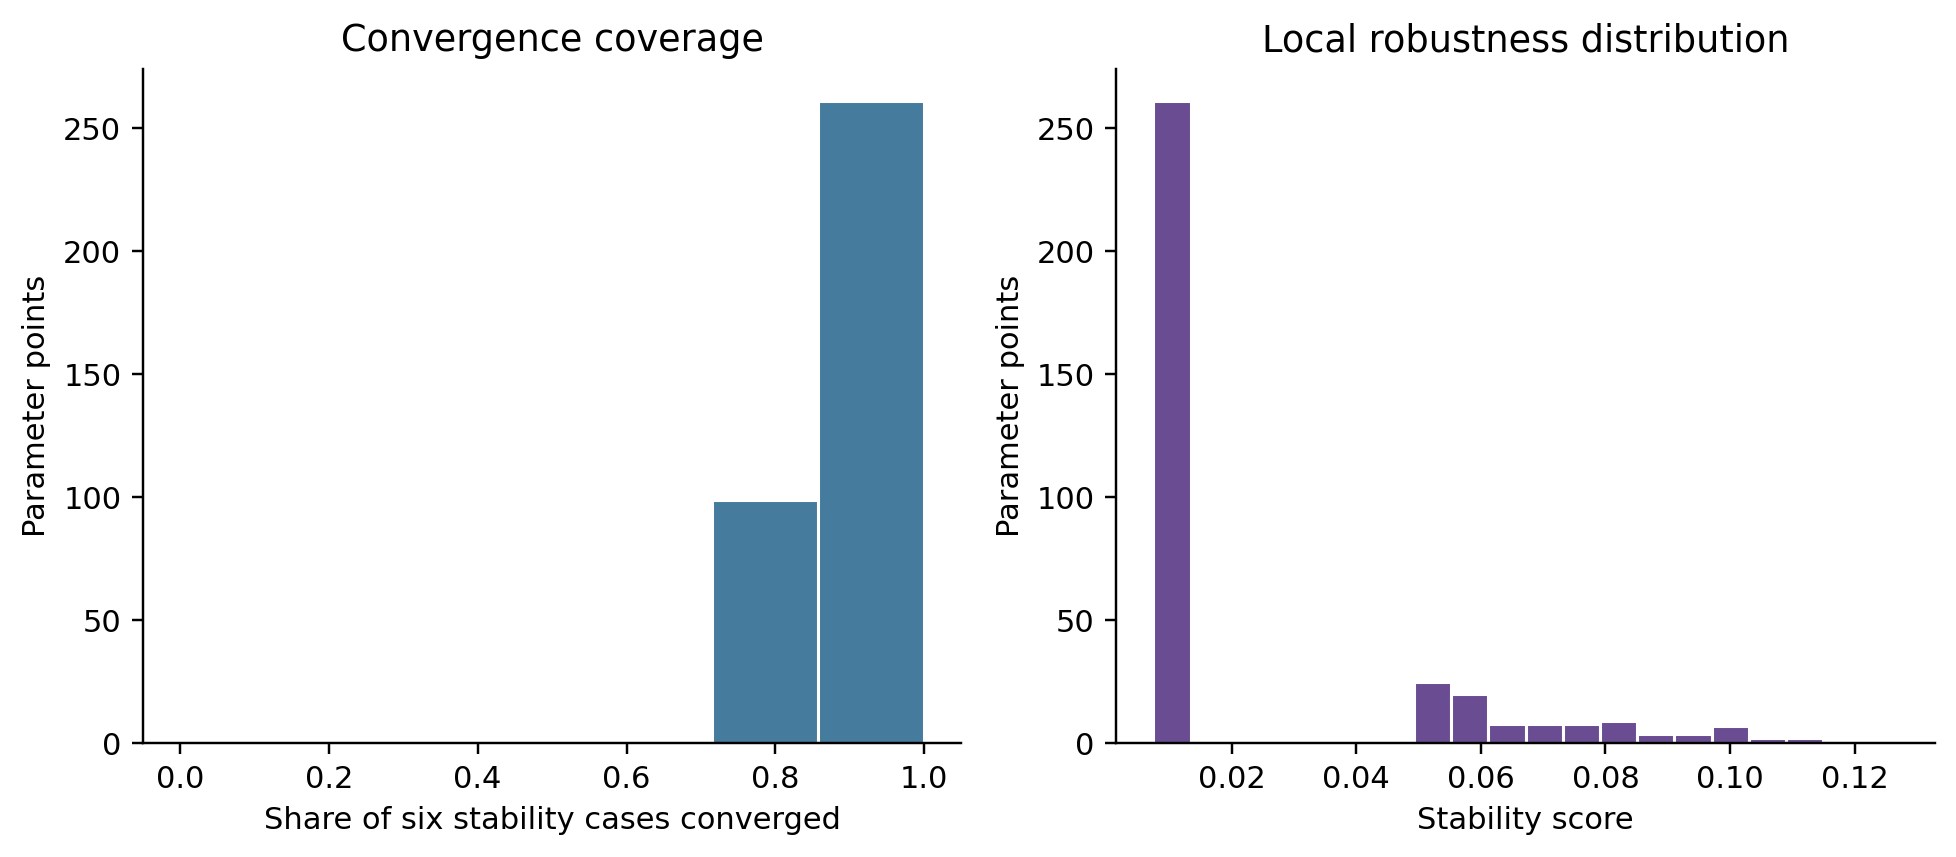
\includegraphics[width=0.92\textwidth]{figure5_stability_distributions.png}
\caption{Coverage of the six convergence cases and distribution of the
continuous stability score. Lower scores indicate smaller tail movement,
spread, and contraction penalties.}
\end{figure}

\section{Economic results}

Across the 360 local configurations, pooled bad-debt-event probability ranged
from 0 to 1.3021\%, with median 0.2604\%. Mean issued credit ranged from 0.1948
to 0.2307 and pause share from 0.4092 to 0.6184. The median pooled credit was
0.2147.

ARS bad-debt probability averaged 0.2951\%, while TRY averaged 0.3935\%. ARS
had no severe-depeg event in this particular common set. TRY severe-depeg
probability stayed close to 20.8\%. Thus, robust convergence of the policy state
does not imply that all exogenous or liquidity-driven failure modes disappear.

\begin{figure}[H]
\centering
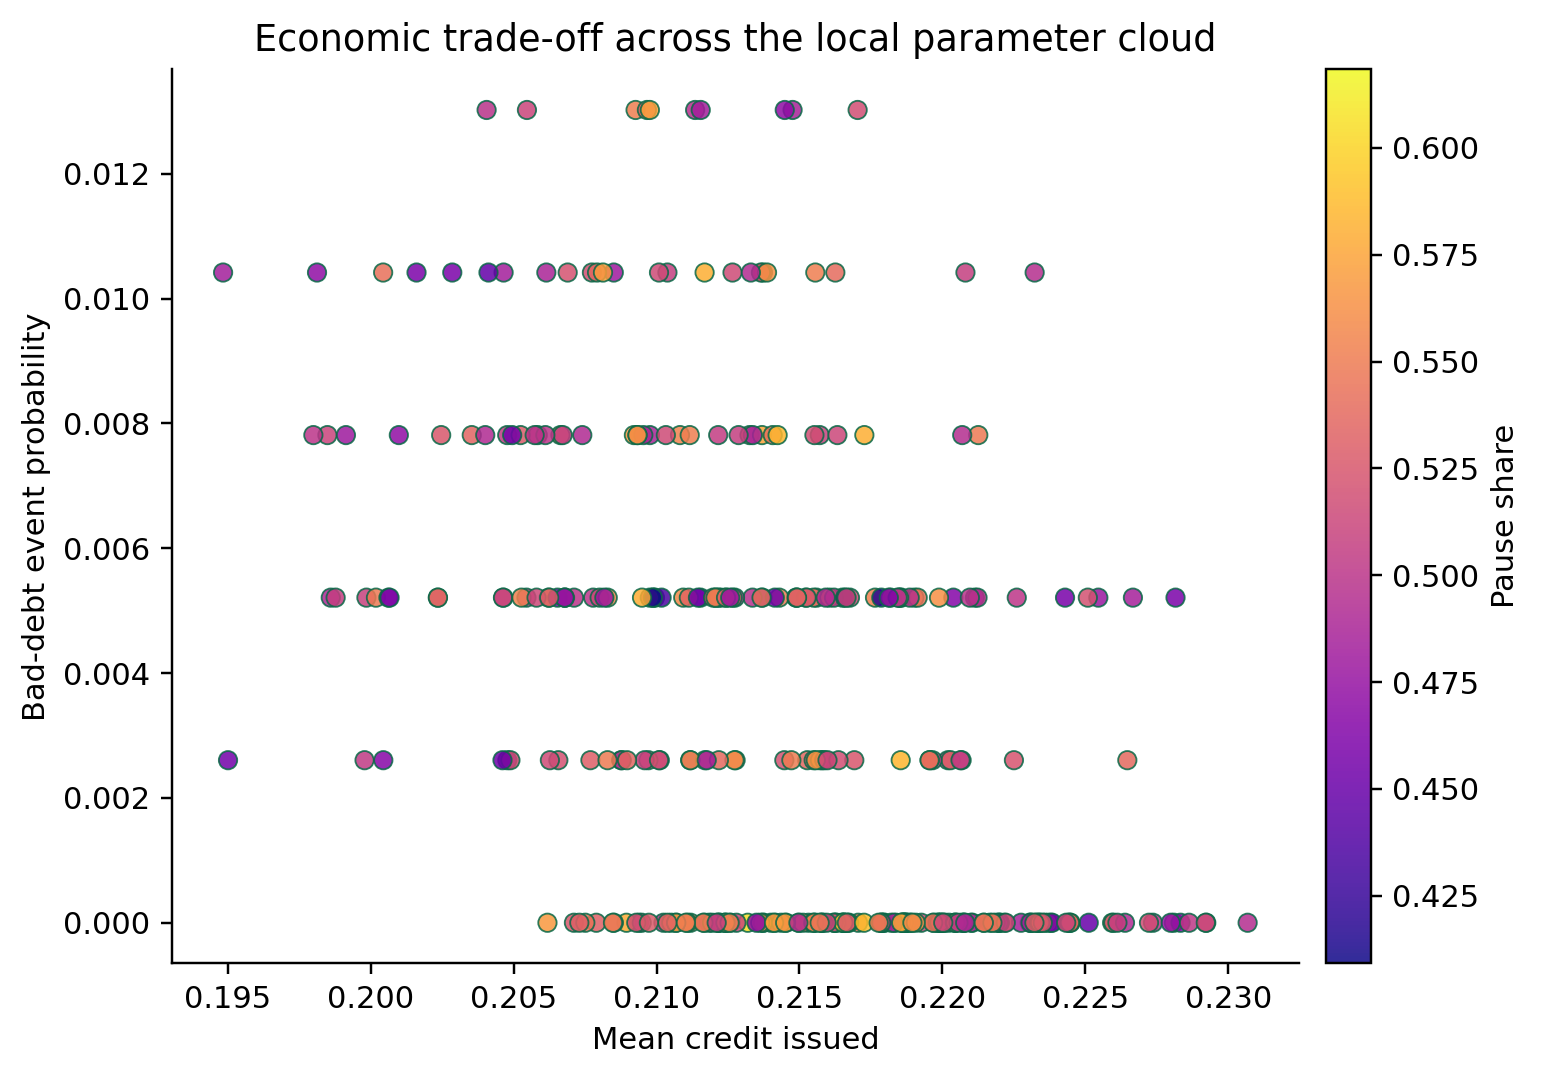
\includegraphics[width=0.86\textwidth]{figure4_economic_tradeoff.png}
\caption{Credit, bad-debt-event probability, and breaker use. Each marker is one
parameter vector evaluated on the same ARS and TRY paths.}
\end{figure}

\subsection{Parameter influence}

Spearman correlations are used as descriptive local sensitivity measures. They
are not structural causal effects and their nominal \(p\)-values are not used as
formal model-selection tests.

\begin{itemize}
\item Ceiling gain versus stability score: \(\rho=0.931\). Within this local
cloud, stronger ceiling response is associated with weaker convergence metrics.
\item Liquidation gain versus bad-debt probability: \(\rho=-0.839\).
\item Rate gain versus pause share: \(\rho=-0.587\).
\item Ceiling gain versus mean credit: \(\rho=-0.550\).
\end{itemize}

\begin{figure}[H]
\centering
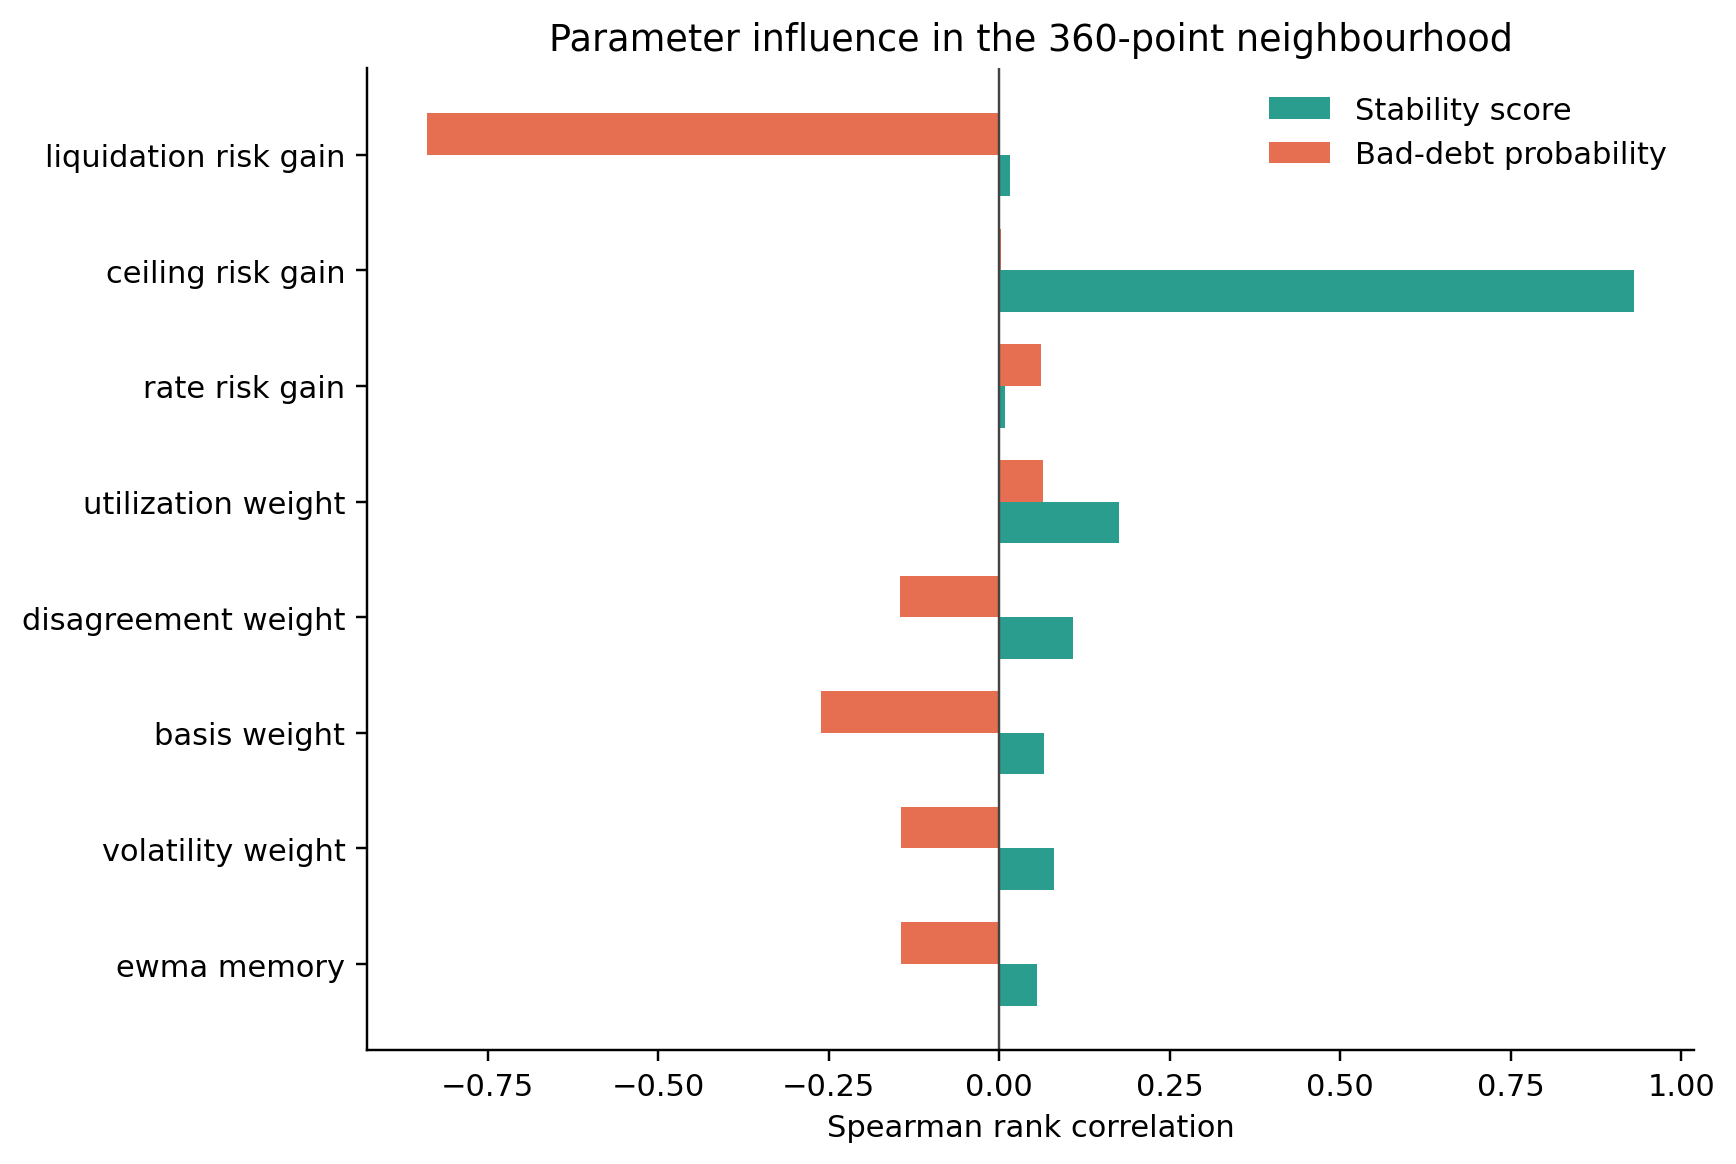
\includegraphics[width=0.94\textwidth]{figure3_parameter_influence.png}
\caption{Local rank correlations with the stability score and bad-debt-event
probability. Signs describe association in the sampled neighbourhood only.}
\end{figure}

\section{Topology of the convergent region}

The eight parameter coordinates are mapped to the unit cube before computing a
Vietoris--Rips filtration. The number of connected components is the zeroth
Betti number \(\beta_0\), while \(\beta_1\) counts one-dimensional cycles at a
given filtration radius.

The stable cloud becomes connected at radius 0.7390. Its largest finite
\(H_1\) lifetime is 0.1844. High-dimensional finite point clouds commonly
produce transient cycles even when sampled from a filled box, so the existence
of cycles alone is not evidence of a genuine hole. We therefore repeat the
maximum-persistence statistic on 30 matched eight-dimensional Latin-hypercube
null clouds.

The null median is 0.1980 and the null 95th percentile is 0.2265. The empirical
tail probability for a null maximum at least as large as the observed value is
\(p=0.9355\). Consequently, the apparent cycles are fully compatible with
finite sampling from a filled region.

\begin{figure}[H]
\centering
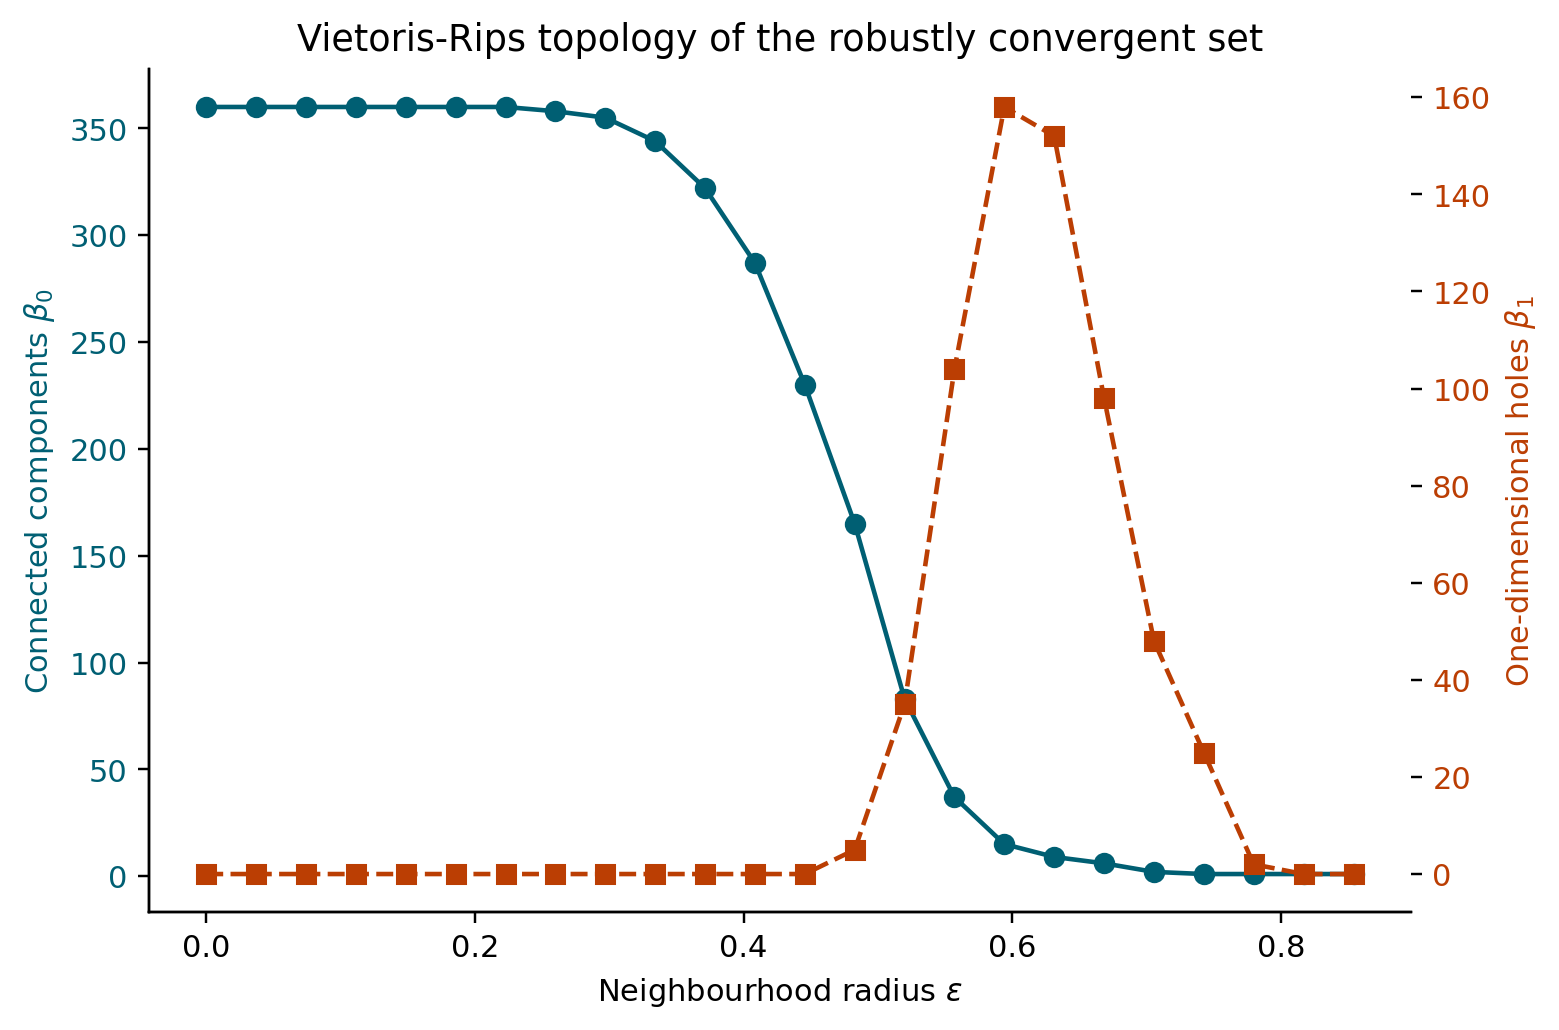
\includegraphics[width=0.88\textwidth]{figure2_betti_curves.png}
\caption{Betti numbers over filtration radius. The point cloud becomes one
component and all sampled \(H_1\) cycles eventually die. The matched null test,
not visual persistence alone, determines whether the cycles are exceptional.}
\end{figure}

The defensible topological conclusion is therefore:
\begin{quote}
The sampled convergent set contains a connected local basin. There is no
evidence of a non-trivial one-dimensional hole beyond the topology generated by
uniform high-dimensional sampling.
\end{quote}
This is not a proof that the global stable set is connected or contractible.

\section{What the experiment establishes}

\begin{itemize}
\item \textbf{Local robustness:} convergence is retained throughout 360
stratified perturbations around the selected centre.
\item \textbf{Non-isolation:} the stable point is part of a measurable local
neighbourhood rather than a single tuned vector.
\item \textbf{Connected sample geometry:} the local stable cloud joins into one
component at a finite filtration scale.
\item \textbf{No exceptional hole:} observed \(H_1\) persistence is smaller than
typical maxima from matched filled-box null clouds.
\item \textbf{Separate safety claim:} convergence and economic outcomes remain
distinct; TRY depeg risk persists in some common paths.
\end{itemize}

\section{Limitations and next proof obligations}

\begin{enumerate}
\item The study is empirical and finite. A Lyapunov or
Lyapunov--Krasovskii argument is still required for a mathematical convergence
theorem, particularly under delay and boundary projection.
\item The reduced stability model preserves signs and bounds but is not identical
to every stochastic mechanism in the full lending simulator.
\item The topology is local and sample-dependent. The broad parameter box may
contain other stable components that the pilot did not resolve.
\item Stability thresholds are explicit design choices. Future work should vary
them and report label sensitivity.
\item Rank correlations can be affected by nonlinear interaction and should not
be read as causal derivatives.
\item A stable equilibrium can still be economically undesirable. Safety,
credit availability, liquidation cost, and depeg resilience require joint
multi-objective evaluation.
\end{enumerate}

\section{Reproducibility map}

\begin{longtable}{>{\raggedright\arraybackslash}p{0.43\textwidth}p{0.49\textwidth}}
\toprule
Repository path & Purpose\\
\midrule
\endhead
\path{analysis/stability_topology.py} & Sampling, reduced-loop stability,
Betti numbers, persistent homology, and influence measures.\\
\path{analysis/run_stability_topology.py} & End-to-end 96+360 point
experiment, full economic runs, CSVs, figures, hashes, and summary.\\
\path{analysis/create_methodology_diagram.py} & Deterministic source for the
publication methodology pipeline in PNG and editable SVG formats.\\
\path{results/stability_topology/pilot_parameter_search.csv} & Broad
96-point search and stability metrics.\\
\path{results/stability_topology/local_360_parameter_results.csv} & All
local parameters, convergence metrics, and pooled economic outcomes.\\
\path{results/stability_topology/economic_results_by_currency.csv} & 720
point--currency records.\\
\path{results/stability_topology/topology_persistence_intervals.csv} & Full
zero- and one-dimensional persistence intervals.\\
\path{results/stability_topology/topology_betti_curves.csv} & Betti numbers
across filtration radius.\\
\path{results/stability_topology/parameter_influence.csv} & Spearman
correlations and nominal \(p\)-values.\\
\path{results/stability_topology/experiment_summary.json} & Seed, bounds,
headline results, topology null test, and SHA-256 output hashes.\\
\path{tests/test_stability_topology.py} & Equation-preservation, sampler,
boundedness, and topology unit tests.\\
\bottomrule
\end{longtable}

\section*{Conclusion}

The 360-point experiment answers the motivating question affirmatively but with
an important qualification. Around the pilot-selected centre, convergence is
stable to simultaneous perturbations of all eight influential coefficients.
The sampled region is connected, and its transient cycles do not exceed those
expected from a uniformly filled eight-dimensional cloud. The result is robust
computational evidence for a local stability basin; it is not yet a global
topological theorem or a formal proof of delayed closed-loop convergence.

\end{document}
